\documentclass[french, 12pt]{article}


\usepackage[utf8]{inputenc}    % Encodage
\usepackage[T1]{fontenc}       % Encodage des polices
\usepackage{lipsum}            % Générateur de texte pour les exemples
\usepackage{graphicx}          % Pour inclure des images
\usepackage{amsmath}           % Pour les formules mathématiques
\usepackage{amsfonts}          % Pour les polices mathématiques
\usepackage{amssymb}           % Pour les symboles mathématiques
\usepackage{hyperref}          % Pour les liens
\usepackage{fancyhdr}          % Pour les en-têtes et pieds de page
\usepackage{xcolor}


% Configuration de l'en-tête et du pied de page
\pagestyle{fancy}
\fancyhf{}
\fancyhead[L]{Sokoban}
\fancyhead[R]{Sacha David et Nathael Carlier}    
\fancyfoot[C]{\thepage}       


% Titre et auteur
\title{Projet Sokoban}
\author{Sacha David et Nathael Carlier\\
       Prép'Isima 2}
\date{\today}








% détaillant la modélisation du jeu (choix retenus pour la modélisation du plateau,
%des éléments ainsi que les strutures de données. À des fins d’évaluations, il sera précisé comment lancer le programme.)
\begin{document}


\maketitle


\tableofcontents


\section{Introduction}


   Le but de ce projet est de recréer le jeu \href{https://fr.wikipedia.org/wiki/Sokoban}{Sokoban} en utilisant le langage de programmation C.


   C'est un jeu ou le joueur doit ranger des caisses sur des cases cibles. Il peut se déplacer dans les quatre directions, et seulement pousser (pas tirer) une seule caisse à la fois. Une fois toutes les caisses rangées, le niveau est réussi et le joueur passe au niveau suivant, plus difficile en général. L'idéal est de réussir avec le moins de déplacements possibles. En principe le personnage de ce jeu est un gardien d'entrepôt rangeant les caisses d'un entrepôt à leur bon endroit. Sokoban ressemble en général à l'illustration ci-dessus (mais comme vous allez le voir nous avons pris quelques libertés de design).


   \begin{figure}[h]
       \centering
       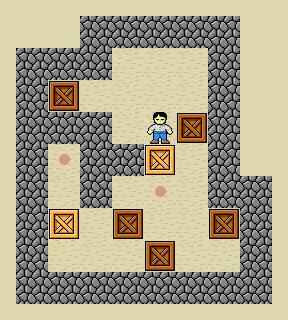
\includegraphics[width=0.4\textwidth]{illustration/base_sokoban.png}
       \caption{Exemple typique d'un jeu sokoban}
   \end{figure}


\section{Nécessaire pour le lancement du jeu}


Pour cette section on vous renvoie sur la \href{../doc/redirect.html}{page d'accueil} de notre documentation expliquant la démarche à suivre pour compiler et exécuter le jeu.


\section{Choix artistique} % Ou D.A. jsp pas quoi mettre


   \subsection{Explication}
       Nous avons remarqué que les graphismes du jeu de base étaient trop basiques et pas forcément jolis. C'est pour cela que nous avons décidé de complètement changer la direction artistique de notre jeu pour donner un côté plus mignon au jeu.


   \subsection{Changements}
       Le personnage ne sera plus un gardien d'entrepôt mais un \href{https://fr.wikipedia.org/wiki/Hydrochoerus_hydrochaeris}{capybara} et lieu dans lequel le jeu ce déroule sera une étendu d'eau en bas d'une casquade. Notre personnage ne déplacera pas de caisse sur leur rangement mais il déplacera des oranges sur des nénuphars.
       De plus les murs en pierre n'existeront pas, ce sera des rochers dépassant de l'eau, le tout avec un rendu en isométrique.
       (Ps: lancez le jeu et vous verrez la diférence)


\section{Structuration du jeu}


   \label{sec:Map}
   \subsection{Grille de jeu}
       La grille de jeu est la carte où le personnage peut se déplacer et interagir avec les éléments présents. Chaque niveau a une carte différente.


       Nous avons décidé de stocker les cartes des niveaux dans des fichiers texte (.txt) différents, ces fichiers sont tous nommés \textcolor{green}{\textit{'map'}} puis leur numéro de niveau. Par exemple \textcolor{green}{\textit{'map1.txt'}} est la carte du premier niveau. \\
       Un fichier est organisé de manière à former un tableau de lettre et d'espace où chaque caractère représente un élément. La position des caractères dans le fichier et dans le jeu seront les mêmes (au début).
       \begin{itemize}
           \item 'W': Wall, représenté par rocher.
           \item 'C': Caisse, représenté par une orange (que le joueur devra pousser).
           \item 'I': Interest point, représenté par un nénuphar (qui accueillera une orange).
           \item 'P': Player, représenté par un Capybara.
           \item 'F': Rocks with Frog, représente un type de rochers particulier.
           \item ' ': Void, ce sont les cases où il y a rien.\\
       \end{itemize}


       Pour l'instant, la grille de jeu présente dans le fichier est inutilisable par un programme. C'est pour ça que l'on va stocker le contenu de celui-ci dans un tableau.


       Mais tout d'abord laissez moi vous présenter la structure qui va accueillir notre grille de jeu et pas que. Nous avons nommé cette structure \href{../doc/html/struct_map.html}{\textcolor{blue}{\underline{Map}}}. Elle contient plusieurs attribut expliqués dans la \href{../doc/html/struct_map.html}{\textcolor{blue}{\textit{documentation}}}, ici nous allons nous concentré sur les attribut utile à l'exécution du jeu et non à l'affichage des textures. \\


       \href{../doc/html/struct_map.html}{\textcolor{blue}{\underline{Map}}} stocke 2 tableaux de 2 dimensions représentant les grilles de jeu. Il y a un tableau stockant tous les éléments du jeu et un autre qui stocke aussi la grille de jeu mais il stocke seulement les cases vides et les points d'intérêts. Le premier tableau représente la carte à tout moment de jeu, ce tableau change à chaque action du joueur. Tandis que le deuxième tableau ne change pas durant toute la partie, en effet il stocke la grille de jeu à l'état initial. Il va servir entre autre de repaire pour vérifier si les points d'intérêts sont complété.\\
       Pour pouvoir correctement lire ces tableaux il faut connaître leur nombre de ligne et colonne, c'est pour ça que \href{../doc/html/struct_map.html}{\textcolor{blue}{\underline{Map}}} stocke ces données. Cette structure stocke aussi le numéro de la carte, cela permet de changer de carte plus facilement.


   \subsection{Joueur}
       La structure \href{../doc/html/struct_map.html}{\textcolor{blue}{\underline{Map}}} vu précédemment suffit à stocker toutes les informations utiles pour le fonctionnement du jeu. Malgré cela nous avons décidé de créer une structure pour représenter le personnage \href{../doc/html/struct_player.html}{\textcolor{blue}{\underline{Player}}}.


       Cette structure stocke principalement des informations utiles à l'affichage du personnage. Malgré cela elle stocke la position du joueur en i et j (y et x pour un plan mathématique). Ce stockage facilite les mouvements du joueur puisque l'on n'a pas besoin de chercher la position du joueur à chacun de ses déplacements.


   \subsection{Interaction}
       Nous avons défini les éléments du jeu et leur structuration, il nous faut dès à présent définir les interactions entre ces éléments.


       Le joueur et les caisses sont les seuls éléments à se déplacer. En effet le principe du jeu \textbf{Sakoban} est de déplacer des boîtes jusqu'à un endroit clé. Pour ce faire, le personnage peut se déplacer et déplacer des caisses. Ces déplacements ont quelques contraintes:


       \begin{itemize}
           \item[$-$] Le joueur ne peut ni traverser de mur ni traverser de caisse (orange).
           \item[$-$] Une caisse a les mêmes contraintes que le joueur.
           \item[$-$] Le joueur et les caisses ne peuvent pas sortir de la carte.
           \item[$-$] Une caisse est déplaçable uniquement par le joueur.
           \item[$-$] Le joueur pousse une caisse dans la direction de son déplacement.
       \end{itemize}


       Pour faire les déplacements et respecter ces contraintes nous avons créé une \href{../doc/html/move_8h.html}{\textcolor{blue}{\underline{fonction}}}. \\
       Pour fonctionner elle a besoin d'avoir le sens vers lequel le joueur veut aller. C'est pour ça que la fonction prend en paramètre un attribut indiquant le sens, définis par l'appui d'une des 4 touches directionnels \textbf{ZQSD}. En fonction du sens donné en paramètre, le personnage va essayer d'aller une case plus loin dans le sens donné à l'intérieur de la grille de jeu.\\

       Avant de déplacer le personnage à l'endroit voulu, on vérifie si, cet emplacement (fait de coordonnées i,j) est dans la carte, si il y a un mur dessus. Dans ces cas-là, le déplacement n'a pas lieu car il est interdit. Mais si il y une boite, il faut vérifier que la case après la boite existe puis si c'est le cas si elle est libre (sans mur). Une fois cela fait, on peut déplacer la caisse dans sa nouvelle case et faire de même avec le personnage. Ce genre de déplacement dans la grille est fait en mettant la caisse ou le joueur, dans la nouvelle case puis remplace celle où elle était par la valeur de cette même case dans le tableau initial.
       Tout ça pour un seul déplacement.


   \subsection{Gestion de niveau}
       \subsubsection{Recommencer}
       Dans le cas où une caisse ne peut plus bouger donc que le niveau est bloqué, ou bien que le joueur a envie de redémarrer le niveau. Il faut une touche ou bouton permettant de le faire.
       Nous avons choisi de faire redémarrer le niveau avec la touche \textbf{R} (pour Recommencer).


       Pour recommencer on relit le fichier correspondant au niveau sur lequel on est, puis on écrase l'instance de la Map actuelle par une nouvelle instance de Map contenant l'état initial de ce niveau.


       \subsubsection{Prochain niveau}


       A chaque fin de niveau, une fois que les objectifs de la carte sont remplis, il faut générer un nouveau niveau donc une nouvelle carte.
       Pour ce faire, on stocke la prochaine map dans une instance de la structure Map puis on écrase les données de l'ancienne carte pour remplacer l'ancienne par la nouvelle.


       Mais, pour savoir quand il faut charger un nouveau, on a besoin de vérifier si un niveau est réussi ou pas. C'est pour ça que l'on a créé une \href{../doc/html/move_8h.html}{\textcolor{blue}{\underline{fonction}}} pour ça.




\section{Affichage du jeu}
% Comment on affiche le tout


% Récap arboresence projet ou pas
\section{Conclusion}






\end{document}





